\subsection{How much spatial resolution is needed}\label{sec:adequate}
Sioux Falls has 24 nodes and 76 arcs in one block atom. Its structural weight condition is therefore the same for every OD, and the connected and unrestricted classifications coincide; the experiments measure variation due to realized responses and heterogeneous marginal costs. The query-dependent classification is illustrated separately in Figure~\ref{fig:blockcut}.

Six input-selected queries away from node 10 change jointly from $0.2$ to $1.6$ times their base values with all other demands fixed and routes responsive; they are the shortest and longest free-flow ODs in each demand tercile (Appendix~\ref{supp:newod}). Table~\ref{tab:newod} reports their ranges. The adaptive rule separates them sharply: the geometric accounts for $(7,18)$ lie in $[642,702]$, their midpoint $672$ has maximum absolute error $30$, or $4.3\%$ of the largest account, and this family admits one common summary at a $5\%$ tolerance; the $(1,19)$ and $(7,12)$ geometric ranges cross zero and require boundary-specific reporting at every tolerance considered below.
\begin{table}[pos=htbp]
\footnotesize
\caption{System contributions and spatial ranges for six prespecified queries,
responsive-background assignment (TSTT units). Connected: all admissible connected regions;
screenline: the geometric family constructed independently of attribution
values. All $C_j$ are positive. Origin-cut accounts, negative shares, and
neighbourhood ranges are retained in Appendix~\ref{supp:newodaccuracy}.}
\label{tab:newod}
\small
\begin{tabular*}{\tblwidth}{@{\extracolsep{\fill}}lrrr}
\toprule
OD & $C_j$ & Connected [min, max] & Screenline [min, max]\\
\midrule
$(7,18)$ & $672.9$ & $[634{,}\ 710]$ & $[642{,}\ 702]$ \\
$(1,19)$ & $50{,}097.7$ & $[-13{,}502{,}\ 24{,}260]$ & $[-2{,}767{,}\ 22{,}124]$ \\
$(4,5)$ & $2{,}826.0$ & $[2{,}396{,}\ 3{,}452]$ & $[2{,}652{,}\ 3{,}176]$ \\
$(1,15)$ & $77{,}403.2$ & $[-8{,}286{,}\ 40{,}540]$ & $[511{,}\ 36{,}621]$ \\
$(6,8)$ & $73{,}964.9$ & $[35{,}307{,}\ 66{,}695]$ & $[45{,}230{,}\ 65{,}286]$ \\
$(7,12)$ & $117{,}482.3$ & $[-17{,}616{,}\ 60{,}029]$ & $[-2{,}967{,}\ 57{,}780]$ \\
\bottomrule
\end{tabular*}
\end{table}

The input-stratified selection experiment widens the view to an
input-only selection of 18 of the 528 positive Sioux Falls OD demands
(Appendix~\ref{sec:coverage} states the rule and reports every query).
Each OD changes alone over $\pm10\%$ and $\pm20\%$ intervals while
other demands remain fixed with endogenous rerouting; the same
36-direction geometric family is used throughout. For each nonempty
family, let $\beta=(\phi_{\max}+\phi_{\min})/2$ and
$\varepsilon=(\phi_{\max}-\phi_{\min})/2$. This common summary
minimizes the largest absolute discrepancy, so every reported boundary
satisfies $|\phi(U)-\beta|\leq\varepsilon$. The reported normalized
error is
\begin{equation}
r_j^{\mathcal F}=100\,\varepsilon_j^{\mathcal F}\Big/\max\bigl(|\phi_{j,\min}^{\mathcal F}|,|\phi_{j,\max}^{\mathcal F}|\bigr),
\label{eq:normerror}
\end{equation}
the absolute deviation of every account from the common value as a
percentage of the family's largest account magnitude; it does not bound
each account's own relative error. We apply a fixed descriptive tolerance
$r_j^{\mathcal F}\leq5\%$; this is a reporting choice rather than a
transport welfare threshold. When all accounts in a family share one
sign, $r_j^{\mathcal F}\leq50\%$, so values near $50\%$ indicate that
the smallest magnitude is far below the largest, not that the accounts
nearly agree.
At $\pm10\%$ and $\pm20\%$, respectively, 1 and 1 of 18 queries meet this tolerance, while 1 and 1 have accounts of both signs; representative common summaries at $\pm20\%$ appear in Appendix~\ref{sec:coverage}.

\begin{figure}[t]\centering
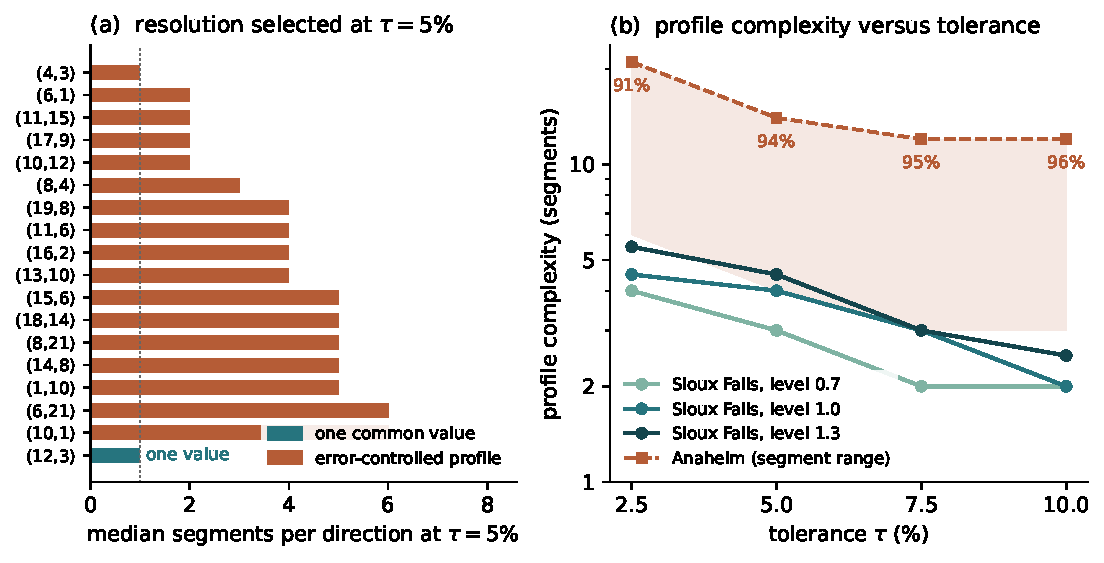
\includegraphics[width=0.99\linewidth]{../figures/fig_v110_summary_frontier.pdf}
\caption{Spatial resolution selected by the error tolerance. Left: the
median minimal segments per projection direction that each of the 18
input-stratified queries receives at the $5\%$ family tolerance
(baseline load; queries sorted by selected resolution; one query is
adequately summarized by a single common value, the remainder by
error-controlled profiles). Right: the profile complexity as the
tolerance varies from $2.5\%$ to $10\%$ --- median segments per
projection direction on Sioux Falls (36 normals, distinct chains
deduplicated, three load levels) and per-query segments on Anaheim's
ordered families; underlying numbers in Table~\ref{tab:tolerance}
(Appendix~\ref{sec:coverage}).}\label{fig:commonsummary}\end{figure}

Figure~\ref{fig:commonsummary} presents the selection and its cost. A
minority of queries admits one common value at a working tolerance;
every other query is summarized one direction at a time. Three counts
should be distinguished when reading these results: the number of
distinct boundary regions $N_{\mathrm{unique}}$, the number of ordered
direction chains $N_{\mathrm{chain}}$ along which they are reported,
and the total number of reported segments $L_{\mathrm{total}}$. On
Sioux Falls the 36 projection normals of the geometric family induce
22--35 distinct ordered chains per query over 1--21 regions each, and
consecutive entries of one chain are nested along that
direction, so the chain --- not the merged sequence --- is the unit of
spatial contiguity; segmenting each chain at the family tolerance
needs a median of $2$--$5.5$ segments per direction across the three
load levels as the tolerance ranges over $2.5$--$10\%$ (at the $5\%$
tolerance and baseline load: median $4$, maximum $8$), with
$L_{\mathrm{total}}$ at a median of $117$ over the distinct chains of
the learned-assignment queries. Per-chain minimality therefore does
not by itself make the delivered representation smaller than the
deduplicated set of boundary values; the direction-resolved profiles
are what the framework delivers there, and the multi-direction counts
quantify direction-specific spatial resolution. Ordering all
directions into one progress sequence yields fewer apparent segments
only by grouping non-adjacent cross-sections, so those counts are not
spatial summaries and are retained only for comparison
(Table~\ref{tab:tolerance}). On Anaheim's single-direction ordered
families --- where the strong compression claims rest --- the same
relaxation raises the compression of the 83--211 accounts
per query from $91.4\%$ (6--21 segments) to $96.4\%$ (3--12
segments). With the same segment count, equal-count partitions have
median worst-segment error $1.4$--$4.0$ times the greedy error per
direction on Sioux Falls and $4.7$--$18.8$ times the tolerance on
Anaheim, so position-aware segmentation is what provides the error
control, not the segment count alone.

The $\pm10\%$ and $\pm20\%$ summaries of the same 18 queries are close in normalized terms, so further subdividing the perturbation width adds little information. The congestion state of the baseline is the more informative axis. All 528 demands are scaled jointly to $0.7$, $1.0$ and $1.3$ times their published values; at each level the level equilibrium is solved once, the focal query alone moves by $\pm20\%$, other demands stay fixed with responsive routes, and the endpoint identity supplies the attribution column (solver protocol in Appendix~\ref{supp:newod}).
\begin{table}[t]\centering\footnotesize
\caption{Common-summary statistics across baseline load levels (18
queries, focal $\pm20\%$, same 36-direction family). Normalized error
is Eq.~\eqref{eq:normerror}; the ratio column is the median
geometric-to-unrestricted spread ratio.}\label{tab:loadlevels}
\begin{tabular}{rrrrrr}\toprule
Level & Queries within $5\%$ & Mixed signs & Median error (\%) & Median ratio & Max.\ negative share\\\midrule
$0.7$ & 2 & 0 & 34.5 & 0.529 & $0.00\%$\\
$1.0$ & 1 & 1 & 44.4 & 0.574 & $0.67\%$\\
$1.3$ & 0 & 3 & 45.2 & 0.563 & $4.03\%$\\
\bottomrule\end{tabular}\end{table}
Table~\ref{tab:loadlevels} shows a monotone pattern: under the light
baseline, accounts are flatter across the family --- the median
normalized error falls to $34.5\%$, two queries satisfy the $5\%$
tolerance and no family crosses zero --- whereas the heavy baseline
makes every query exceed the tolerance, three families mix signs and
the negative share of $(6,21)$ reaches $4\%$. Per-query normalized
errors rise from the light to the heavy level for 17 of 18 queries
(e.g.\ $(10,12)$: $18.6\to35.2\to40.3$; $(1,10)$: $31.2\to44.8\to48.0$).
Across the load levels, light-load conditions admit transferable single
summaries more often, and heavy-load conditions require
boundary-specific reporting. The load-level trend has a theory-side
counterpart: the node-imbalance norm $\norm{d_j}_2$ rises by a factor
of $13.2$ from the light to the heavy baseline, and Eq.~\eqref{eq:cutspread}
sums that imbalance into the spatial range
(Appendix~\ref{sec:coverage} reports the rank correlations and the
Cauchy--Schwarz comparison).

\paragraph{How much does the model-specific level buy?}\label{sec:levelsdiag}
On the synthetic network of Figure~\ref{fig:blockcut}, restricting
attention to the model's path-feasible response envelope restores
boundary consistency despite off-path weight heterogeneity, so the
model-specific level certifies a common account that the universal
condition denies. On Sioux Falls and Anaheim the path-feasible
response envelopes are sufficiently rich that the structural and
model-specific tests both reject a single universal boundary value,
and the diagnosis is stable across load levels
(Appendix~\ref{supp:levelsdiag} reports the numerical diagnosis of the
transferability hierarchy). The realized error-controlled profiles
therefore become the operative representation, and the summaries of
Table~\ref{tab:newod} carry the reporting.
